\cohead{\Large\textbf{Ganzrationale Funktionen}}
\fakesubsection{Ganzrationale Funktionen}
\begin{minipage}{0.66\textwidth}
	Aus einem quadratischen Stück Pappe der Größe  21cm auf 21cm soll ein oben offener Kasten hergestellt werden. Die Ecken mit der variablen Seitenlänge x sind hierzu entsprechend der Abbildung abzuschneiden und die Seiten an den gepunkteten Linien hochzubiegen.
\end{minipage}
\begin{minipage}{0.33\textwidth}
	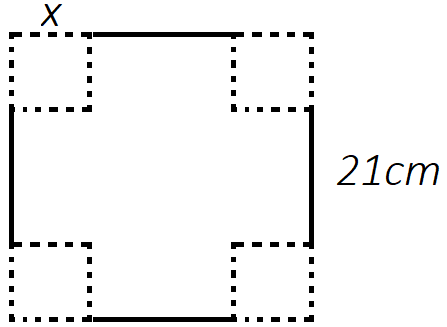
\includegraphics[width=.95\textwidth]{\ganzFkt/pics/einfuehrungKasten.png}
\end{minipage}

\bigskip

\begin{enumerate}[label=\alph*)]
	\item Gib drei verschiedene mögliche Abmessungen (Länge, Breite, Höhe) eines solchen Kastens an und berechne jeweils das zugehörige Volumen.
	\item Beschreibe das Volumen \(V\) des Kastens in Abhängigkeit von der Höhe \(x\) mit einer Gleichung.
	\item Zeichne das Schaubild der Funktion \(V(x)\) im Intervall \(0 \leq x \leq 13\) mit Hilfe deines Taschenrechners und einer Wertetabelle.
	\item Bestimme eine sinnvolle Definitionsmenge für die Funktion.
	\item Für welche Höhe x ist das Volumen des Kastens am größten?
\end{enumerate}

\bigskip

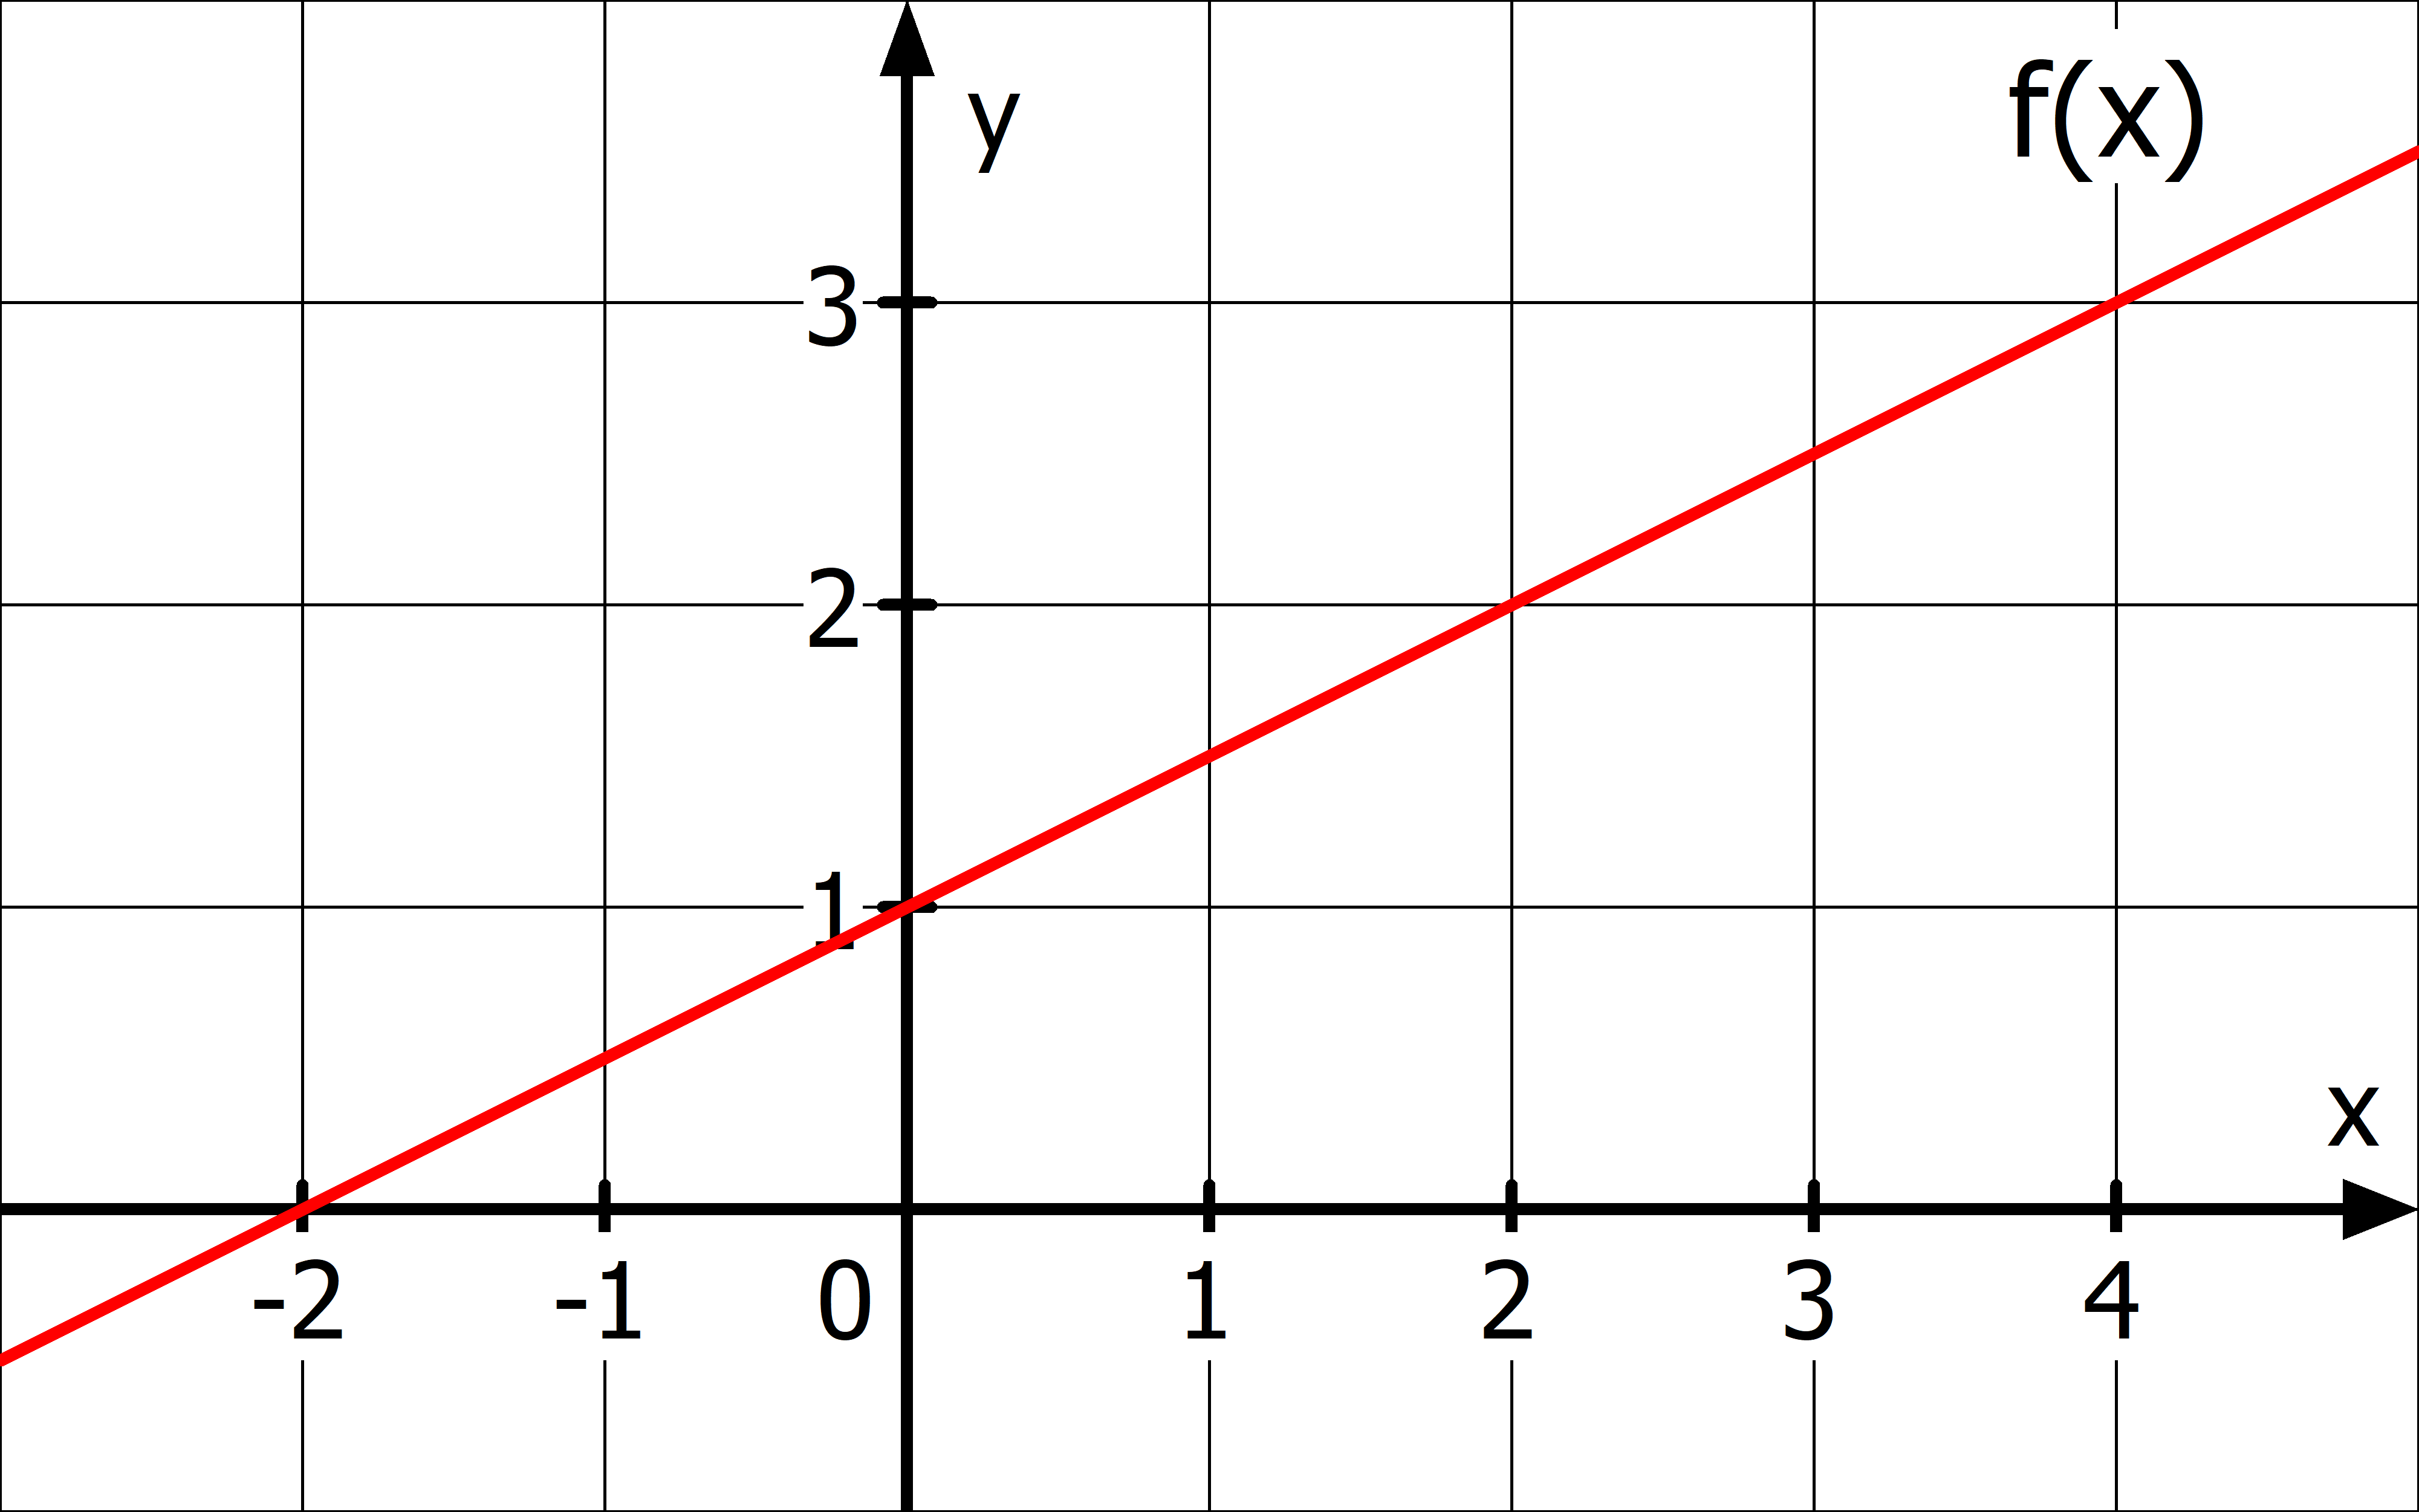
\includegraphics[width=\textwidth]{\ganzFkt/pics/einfuehrung.png}
\newpage
\begin{enumerate}[label=\alph*)]
	\item Mögliche Beispiele: \(V_1=5\cdot \left(21-10\right)\left(21-10\right)=605\)
	
	\hphantom{Mögliche Beispiele: }\(V_2=3\cdot \left(21-6\right)\left(21-6\right)=675\)
	
	\hphantom{Mögliche Beispiele: }\(V_3=8\cdot \left(21-16\right)\left(21-16\right)=200\)
	\item Die Höhe des Kastens entspricht \(x\), während die Länge und Breite jeweils \(21-2x\) entsprechen.
	
	Damit ergibt sich für das Volumen:
	
	\(V(x)=\text{Länge}\cdot \text{Breite}\cdot \text{Höhe}=x\cdot \left(21-2x\right)\left(21-2x\right)=x\left(21-2x\right)^2=4x^3-42x^2+441x\)
	\item
	Schaubild der Funktion\\
	\begin{minipage}{\linewidth}
		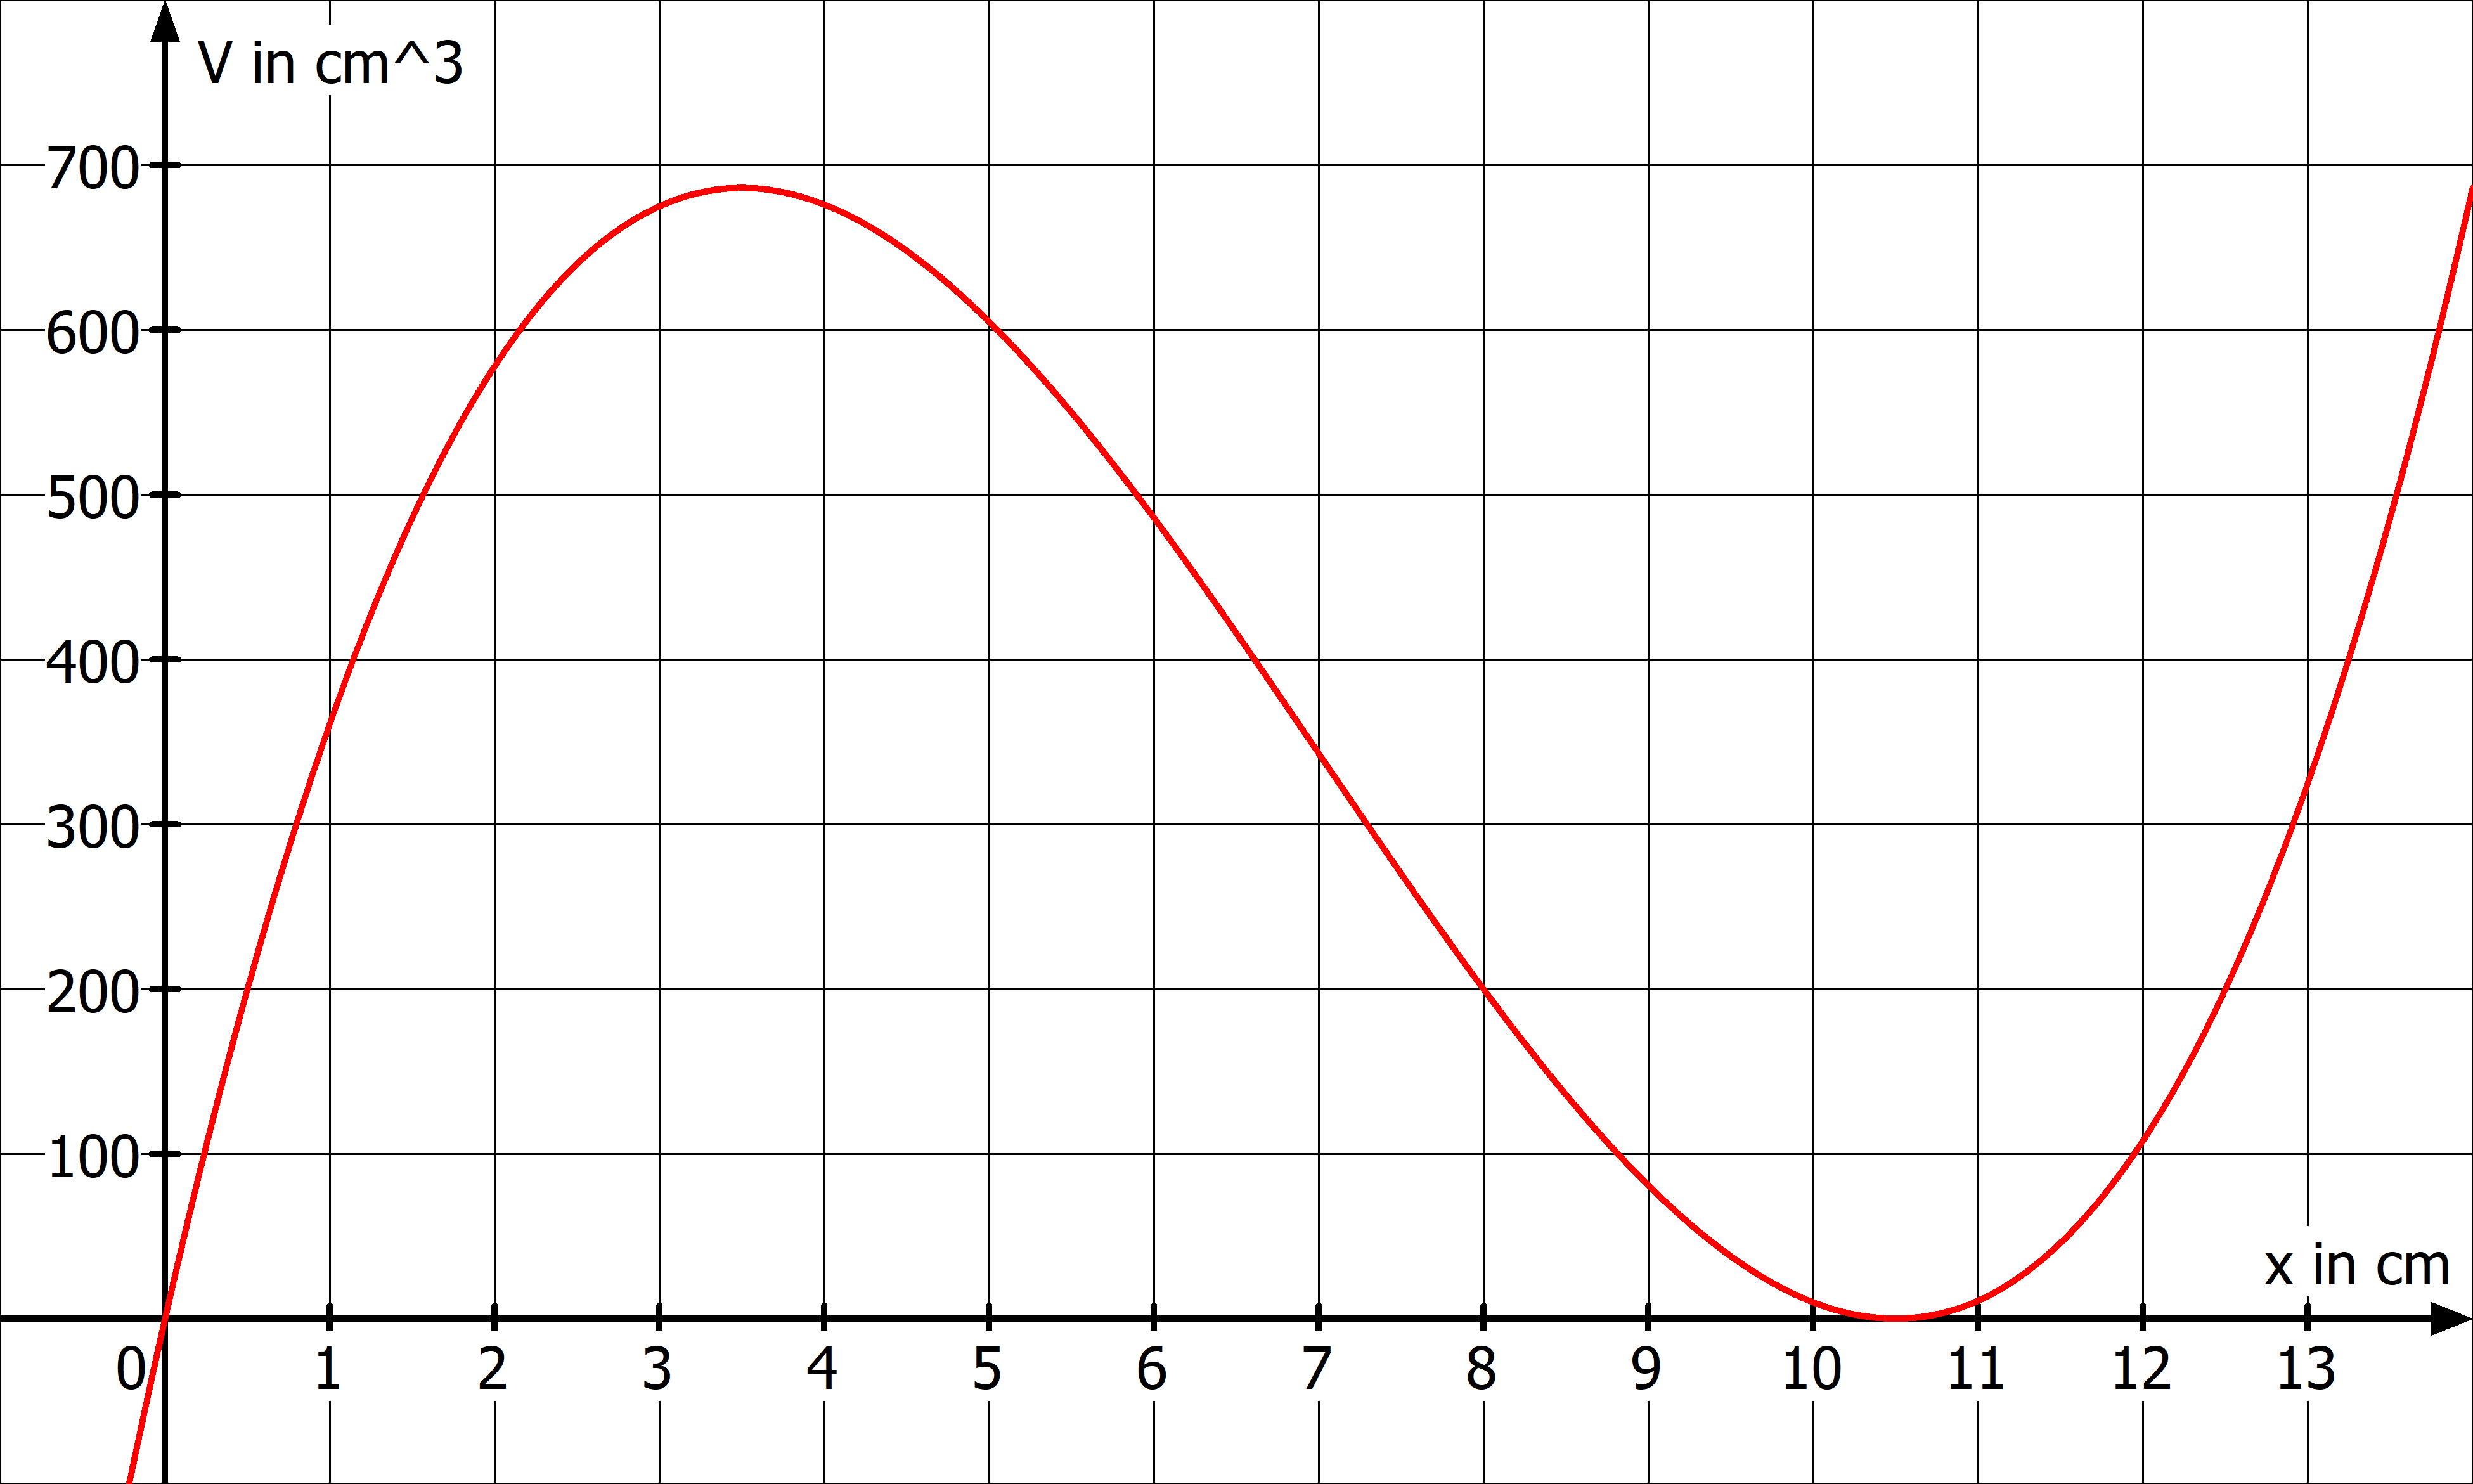
\includegraphics[width=\linewidth]{\ganzFkt/pics/einfuehrungLoes.png}
	\end{minipage}
	
	\item Die Definitionsmenge \(D\) gibt an, welche Werte für \(x\) man einsetzen darf. In diesem Fall sollte \(x\) größer als Null sein, da sonst kein Kasten entsteht und kleiner als \(10,5\) sein, da bei \(x=10,5\) die vier Quadrate das komplette Stück Pappe abdecken:
	
	\(D=]0;10,5[\) oder \(D=\{x\in\R \vert 0< x < 10,5\}\)
	\item Aus dem Schaubild lässt sich ablesen, dass das maximale Volumen ungefähr bei \(x=3,5\) erreicht wird und damit  \(V_{max}=V(3,5)=686\) gilt. Das maximale Volumen lässt sich mit der Ableitung exakt bestimmen, die wir zu einem späteren Zeitpunkt behandeln werden.
\end{enumerate}